\begin{IEEEbiography}[{
    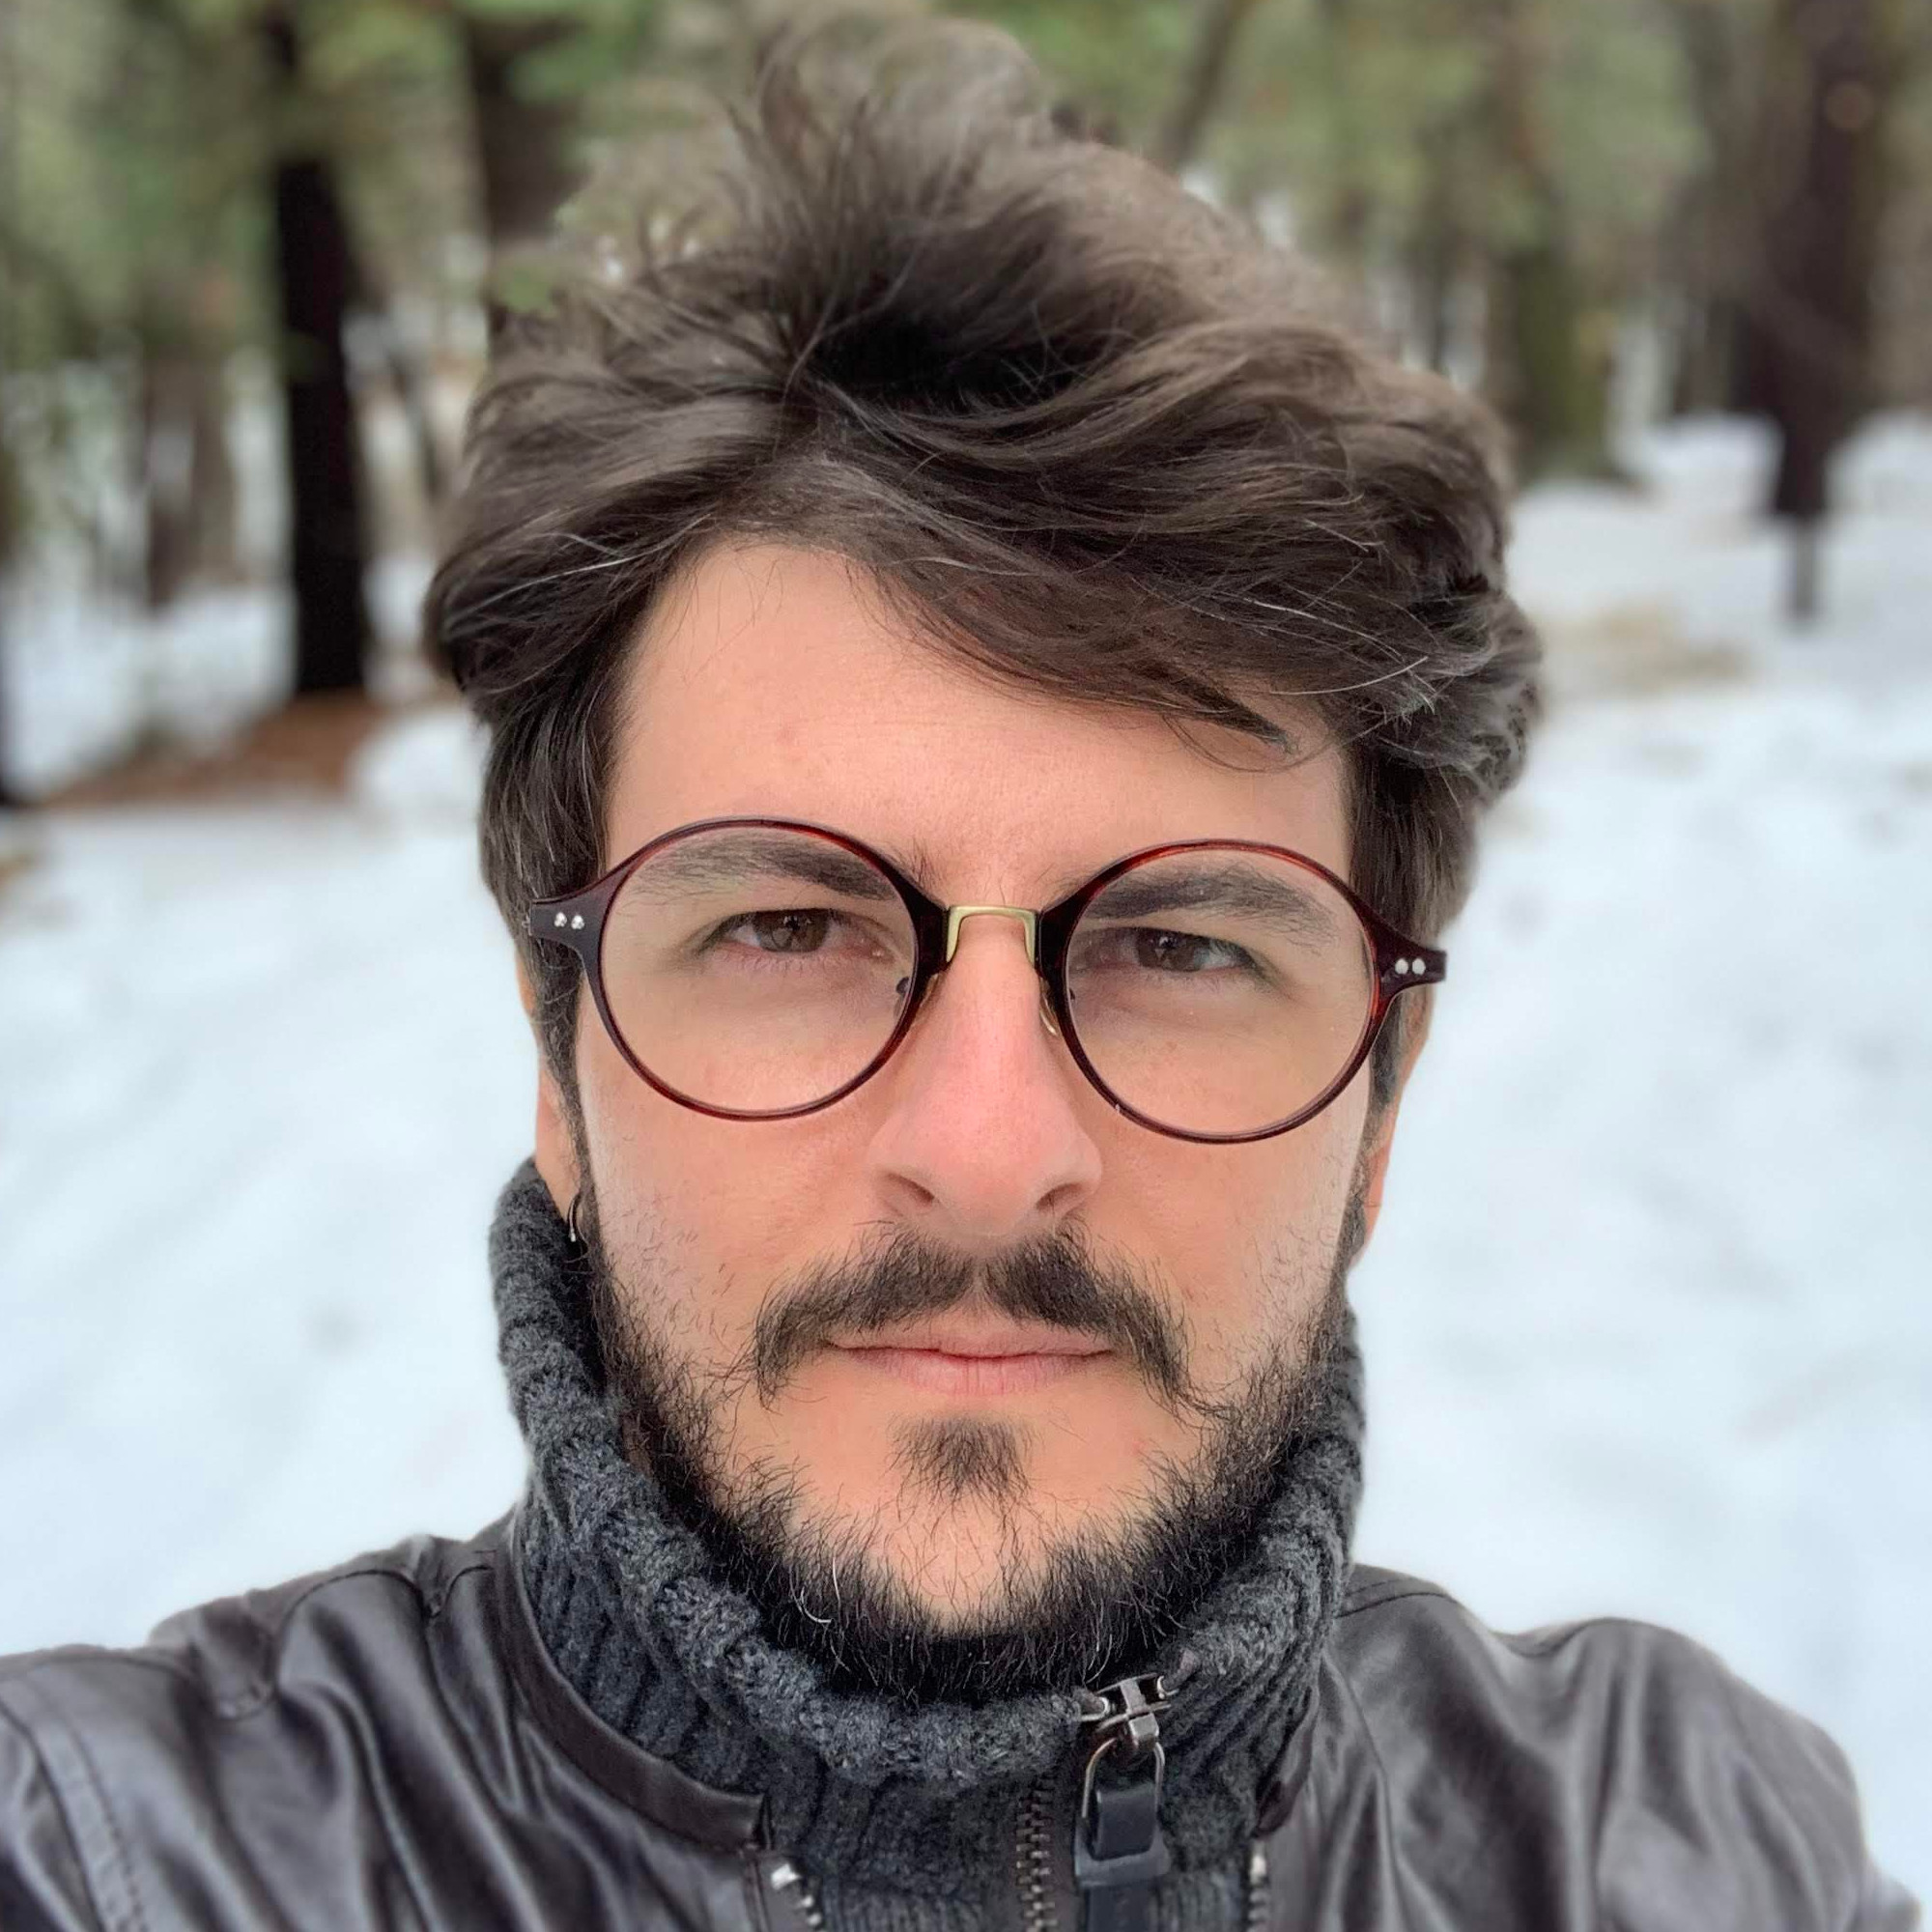
\includegraphics[width=0.8\linewidth,clip,keepaspectratio]{figures/pantuza-bio.jpg}}]{Gustavo Pantuza}
    PhD candidate in Computer Science at the Federal University of Minas Gerais. His research areas are networks, distributed systems and observability.
\end{IEEEbiography}

\begin{IEEEbiography}[{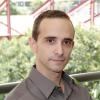
\includegraphics[width=0.8\linewidth,clip,keepaspectratio]{figures/flip-bio.jpg}}]{Luiz Vieira}
is a Professor of Computer Science at the Universidade Federal de Minas Gerais (UFMG). He received his undergraduate and M.S. at the Universidade Federal de Minas Gerais in Belo Horizonte, and Ph. D. degree in Computer Science from the University of California Los Angeles (UCLA). His research interest is in Computer Networking.
\end{IEEEbiography}

\begin{IEEEbiography}[{
    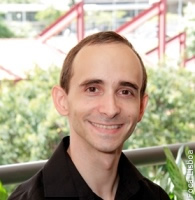
\includegraphics[width=1in,height=1.in,clip]{figures/flop-bio.jpg}}]{Marcos A. M. Vieira} is an Associate Professor of Computer Science at the Universidade Federal de Minas Gerais (UFMG) since 2011. He is awarded a research productivity scholarship level 1 from CNPq. He received his B.Sc. from UFMG in 2002, his M.S. from UFMG in 2004, and his Ph.D. in Computer Science from the University of Southern California (USC) in 2010. Marcos was a Visiting Research Scholar at University of Southern California from 2018 to 2019. His research interests are in Computer Networking and Wireless Networks. He is also a member of IEEE and ACM research communities.
\end{IEEEbiography}
